\documentclass[conference]{IEEEtran}

% ------------------------------------------------
% Fonts & core packages (IEEE-compliant)
% ------------------------------------------------
\usepackage{newtxtext,newtxmath} % Times New Roman text & math
\usepackage{graphicx}
\usepackage{amsmath}
\usepackage{cite}                % compressed numeric citations like [1]–[3]
\usepackage{url}
\usepackage{microtype}
\usepackage{booktabs}
\usepackage{multirow}
\usepackage{hyperref}

% ------------------------------------------------
% Paragraph formatting (one "tab" indent; no extra spacing)
% ------------------------------------------------
\setlength{\parindent}{1em}
\setlength{\parskip}{0pt}

\def\BibTeX{{\rm B\kern-.05em{\sc i\kern-.025em b}\kern-.08em
    T\kern-.1667em\lower.7ex\hbox{E}\kern-.125emX}}

\begin{document}

% ------------------------------------------------
% Title & Authors
% ------------------------------------------------
\title{\fontsize{24pt}{28pt}\selectfont
An Interpretable Hybrid Deep Learning System for Glaucoma Detection Using Retinal Fundus Images with Structural Analysis and Grad-CAM Explainability
}

\author{
\begin{minipage}[t]{0.31\textwidth}
\centering
\fontsize{9pt}{11pt}\selectfont Sourajit Majumder\\
\textit{[Dept. of Computer Science \& Engg. (AI \& ML)]}\\
Narula Institute of Technology\\
Agarpara, Kolkata 700109, India\\
\textup{Email: [sourajitm19@gmail.com]}
\end{minipage}
\hfill
\begin{minipage}[t]{0.31\textwidth}
\centering
\fontsize{9pt}{11pt}\selectfont Kishalay Bairagi\\
\textit{Dept. of Computer Science \& Engg. (AI \& ML)}\\
Narula Institute of Technology\\
Agarpara, Kolkata 700109, India\\
\textup{Email: kishalayb29@example.com}
\end{minipage}
\hfill
\begin{minipage}[t]{0.31\textwidth}
\centering
\fontsize{9pt}{11pt}\selectfont Eshita Biswas\\
\textit{Dept. of Computer Science \& Engg. (AI \& ML)}\\
Narula Institute of Technology\\
Agarpara, Kolkata 700109, India\\
\textup{Email: eshita@example.com}
\end{minipage}
\\[1em]
\begin{minipage}[t]{0.45\textwidth}
\centering
\fontsize{9pt}{11pt}\selectfont Ritika Dutta\\
\textit{Dept. of Computer Science \& Engg. (AI \& ML)}\\
Narula Institute of Technology\\
Agarpara, Kolkata 700109, India\\
\textup{Email: ritika@example.com}
\end{minipage}
\hfill
\begin{minipage}[t]{0.45\textwidth}
\centering
\fontsize{9pt}{11pt}\selectfont Prasun Kumar Jha\\
\textit{Dept. of Computer Science \& Engg. (AI \& ML)}\\
Narula Institute of Technology\\
Agarpara, Kolkata 700109, India\\
\textup{Email: prasun@example.com}
\end{minipage}
}

\maketitle

% ────────────────────────────────────────────────────────────────────% ─────────────────────────────────────────────────────────────────────
\begin{abstract}
Glaucoma is a leading cause of irreversible blindness worldwide,
yet it remains significantly underdiagnosed due to the requirement
for specialist fundus image interpretation. This paper presents an
interpretable hybrid deep learning system for automated glaucoma
detection using retinal fundus images. The proposed approach combines
transfer learning (ResNet18), structural optic disc and cup
segmentation (U-Net), and gradient-weighted class activation mapping
(Grad-CAM) for clinical explainability. Three publicly available
datasets were used for evaluation: ACRIMA (705~images), RIM-ONE~DL
(485~images), and EyePACS-AIROGS-light-v2 (3,540~images), yielding
a combined test set of 1,050 samples. A systematic comparison was
conducted between classical machine learning baselines (Logistic
Regression, SVM-RBF, Random Forest) and deep learning architectures
(ResNet18, EfficientNet-B0). An ablation study evaluated four fusion
strategies combining CNN predictions with handcrafted features and
U-Net-derived cup-to-disc ratio (CDR). The proposed CNN+CDR hybrid
model achieved an area under the receiver operating characteristic
curve (AUC) of 0.9468, sensitivity of 0.9300, and specificity of
0.8018 on the held-out test set, significantly outperforming the
best classical ML baseline (SVM-RBF, AUC\,=\,0.789,
$Z\!=\!10.11$, $p < 0.0001$, DeLong's test; $\chi^2\!=\!98.94$,
$p < 0.0001$, McNemar's test). The U-Net achieved Dice coefficients
of 0.968 and 0.880 for optic disc and cup segmentation respectively
on DRISHTI-GS1. Grad-CAM visualisations confirmed consistent model
attention on the clinically relevant optic disc region, supporting
clinical trustworthiness. The ablation study demonstrated that
U-Net-derived CDR provides complementary structural information to
the CNN (AUC gain: $+$0.002), while handcrafted SVM features are
subsumed by the CNN's learned representations.
\end{abstract}
 
\begin{IEEEkeywords}
Glaucoma detection, retinal fundus imaging, deep learning,
transfer learning, ResNet18, U-Net, cup-to-disc ratio,
Grad-CAM, explainable AI, medical image analysis.
\end{IEEEkeywords}
 
% ─────────────────────────────────────────────────────────────────────
\section{Introduction}
 
Glaucoma affects approximately 80 million people globally and is
the second leading cause of blindness after cataracts~\cite{tham2014}.
Unlike other blinding conditions, glaucomatous vision loss is
irreversible once it occurs; however, early detection and treatment
can halt progression in the majority of cases~\cite{weinreb2004}.
The primary clinical indicator is enlargement of the optic cup
relative to the optic disc, quantified as the cup-to-disc ratio
(CDR). A CDR exceeding 0.65 is generally considered indicative of
glaucomatous structural damage~\cite{jonas1988}.
 
Automated analysis of retinal fundus photographs offers a scalable
and cost-effective approach to population-level glaucoma screening.
However, several challenges persist: glaucoma indicators are
spatially localised to the optic disc region; global image
classifiers introduce peripheral noise that can mislead predictions;
and most existing deep learning models lack clinical interpretability,
limiting clinician trust and adoption.
 
Existing approaches fall into three broad categories:
(1)~classical machine learning on handcrafted
features~\cite{niemeijer2007}; (2)~end-to-end deep convolutional
neural networks~\cite{chen2015}; and (3)~segmentation-based methods
that explicitly extract structural features~\cite{orlando2020}.
Few works integrate all three components into a unified,
interpretable system, and most studies evaluate on a single dataset,
limiting generalisability claims.
 
This paper makes four primary contributions:
\begin{enumerate}
  \item A systematic multi-dataset evaluation comparing classical ML
  and deep learning approaches across three heterogeneous publicly
  available datasets, with statistical significance testing using
  both DeLong's AUC test and McNemar's test.
  \item A U-Net-based optic disc and cup segmentation pipeline
  achieving Dice coefficients of 0.968 and 0.880 respectively on
  DRISHTI-GS1, enabling reliable CDR extraction across datasets.
  \item A principled ablation study identifying CNN+CDR as the
  optimal fusion strategy, demonstrating that U-Net-derived
  structural features provide complementary information to deep
  visual features while handcrafted features are redundant.
  \item Grad-CAM explainability analysis quantitatively validating
  that the model attends to clinically relevant optic disc regions,
  supporting trustworthy deployment.
\end{enumerate}
 
% ─────────────────────────────────────────────────────────────────────
\section{Related Work}
 
\subsection{Classical Machine Learning Approaches}
Early automated glaucoma detection systems relied on handcrafted
features including colour histograms, texture descriptors such as
Local Binary Patterns (LBP)~\cite{ojala2002}, and geometric optic
disc measurements. Niemeijer et al.~\cite{niemeijer2007} demonstrated
that CDR extracted from manual segmentation, combined with a linear
discriminant classifier, could achieve competitive screening
performance. However, these methods require careful feature
engineering and are sensitive to image quality variation across
different fundus camera devices.
 
\subsection{Deep Learning for Glaucoma Detection}
CNN-based approaches have increasingly dominated the literature
since 2015. Chen et al.~\cite{chen2015} demonstrated that fine-tuned
AlexNet outperformed classical baselines on the ORIGA dataset.
More recently, transformer-based architectures and attention
mechanisms have shown further improvements~\cite{li2021}. However,
most studies evaluate on a single proprietary dataset, raising
questions about generalisability, and the majority do not provide
clinical explainability.
 
\subsection{Segmentation-Based Methods}
The REFUGE Challenge~\cite{orlando2020} established U-Net variants
as the leading approach for optic disc and cup segmentation, with
top-performing methods achieving Dice coefficients exceeding 0.95
for disc and 0.85 for cup. CDR computed from predicted masks
correlates well with expert clinical measurement~\cite{fumero2011},
providing a structurally grounded complement to image-level
classifiers.
 
\subsection{Explainability in Medical AI}
Selvaraju et al.~\cite{selvaraju2017} proposed Grad-CAM as a
class-discriminative visualisation technique applicable to any CNN.
Its application to retinal disease detection has shown that models
attending to clinically relevant regions generalise better and are
more readily accepted by clinicians in prospective
studies~\cite{jiang2019}.
 
% ─────────────────────────────────────────────────────────────────────
\section{Datasets}
 
Three publicly available fundus image datasets were used for
classification, and one for segmentation.
Table~\ref{tab:datasets} summarises their key statistics.
 
\begin{table}[htbp]
\caption{Datasets Used in This Study}
\label{tab:datasets}
\centering
\begin{tabular}{lcccc}
\toprule
\textbf{Dataset} & \textbf{Images} & \textbf{Glaucoma}
  & \textbf{Normal} & \textbf{Task} \\
\midrule
ACRIMA~\cite{diaz2019}           & 705   & 396 & 309 & Classification \\
RIM-ONE DL~\cite{rimone}         & 485   & 172 & 313 & Classification \\
EyePACS-AIROGS~\cite{airogs}     & 3,540 & 770 & 770 & Classification \\
DRISHTI-GS1~\cite{sivaswamy2015} & 50    & —   & —   & Segmentation   \\
\bottomrule
\end{tabular}
\end{table}
 
\textbf{ACRIMA} contains 705 fundus images labelled by two
glaucoma specialists; the class label is encoded in the
filename (\texttt{\_g\_} denotes glaucoma). \textbf{RIM-ONE~DL}
provides 485 images from three Spanish hospitals with predefined
\texttt{Glaucoma/} and \texttt{Normal/} subdirectory splits.
\textbf{EyePACS-AIROGS-light-v2} is a large-scale challenge dataset
with predefined train/validation/test splits; a stratified cap of
1,000 images per class was applied to the training split to balance
computational cost. \textbf{DRISHTI-GS1} provides 50 training images
with expert soft segmentation masks and pre-computed mean CDR values
from four raters; it was used exclusively for U-Net training and CDR
proxy validation.
 
For classification, all three datasets were merged and partitioned
into train (70\%), validation (15\%), and test (15\%) using stratified
random sampling (seed\,=\,42). The test split was held out until
final evaluation.
 
\begin{figure}[htbp]
  \centering
  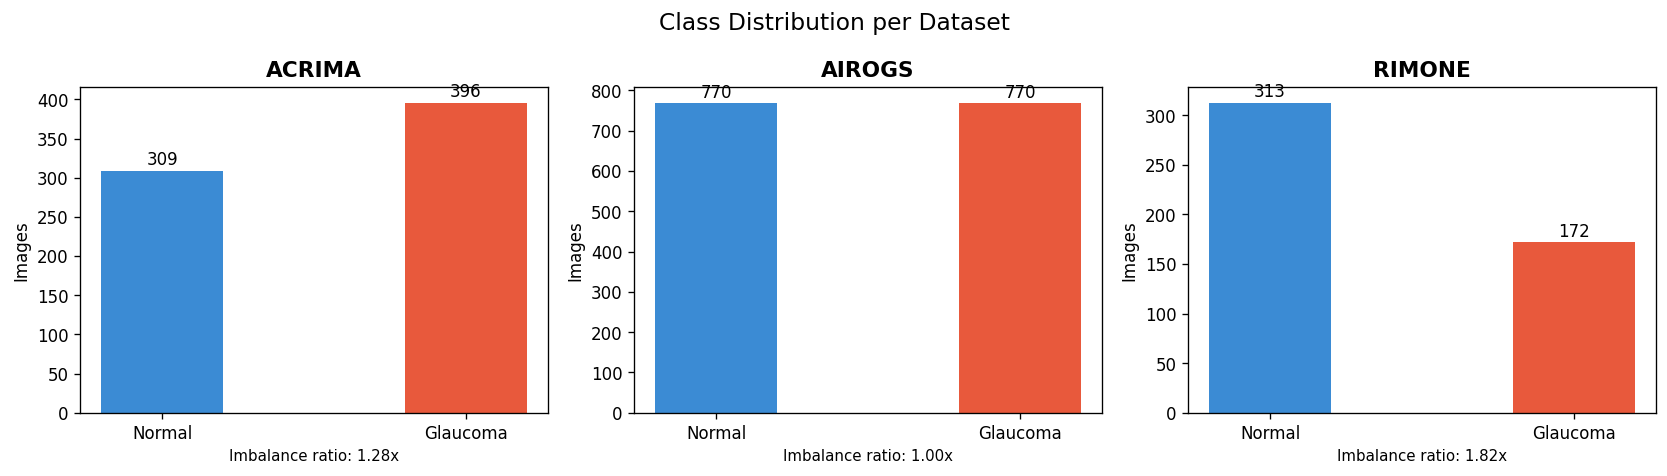
\includegraphics[width=0.46\textwidth]{class_distribution.png}
  \caption{Class distribution across the three classification
    datasets prior to train/test splitting.}
  \label{fig:class_dist}
\end{figure}
 
% ─────────────────────────────────────────────────────────────────────
\section{Methodology}
 
\subsection{Preprocessing Pipeline}
All fundus images underwent the following standardised pipeline:
\begin{enumerate}
  \item \textbf{CLAHE}: Contrast Limited Adaptive Histogram
  Equalisation on the L channel in LAB colour space (clip
  limit\,=\,2.0, tile\,=\,$8\!\times\!8$) to enhance optic
  disc visibility.
  \item \textbf{Circular masking}: Otsu-threshold detection
  of the fundus boundary; non-retinal background zeroed out.
  \item \textbf{Resizing}: $224\!\times\!224$ px (Lanczos) for
  CNN; $256\!\times\!256$ px for U-Net.
  \item \textbf{Normalisation}: ImageNet statistics
  ($\mu\!=\![0.485,\,0.456,\,0.406]$,
   $\sigma\!=\![0.229,\,0.224,\,0.225]$).
\end{enumerate}
 
\begin{figure}[htbp]
  \centering
  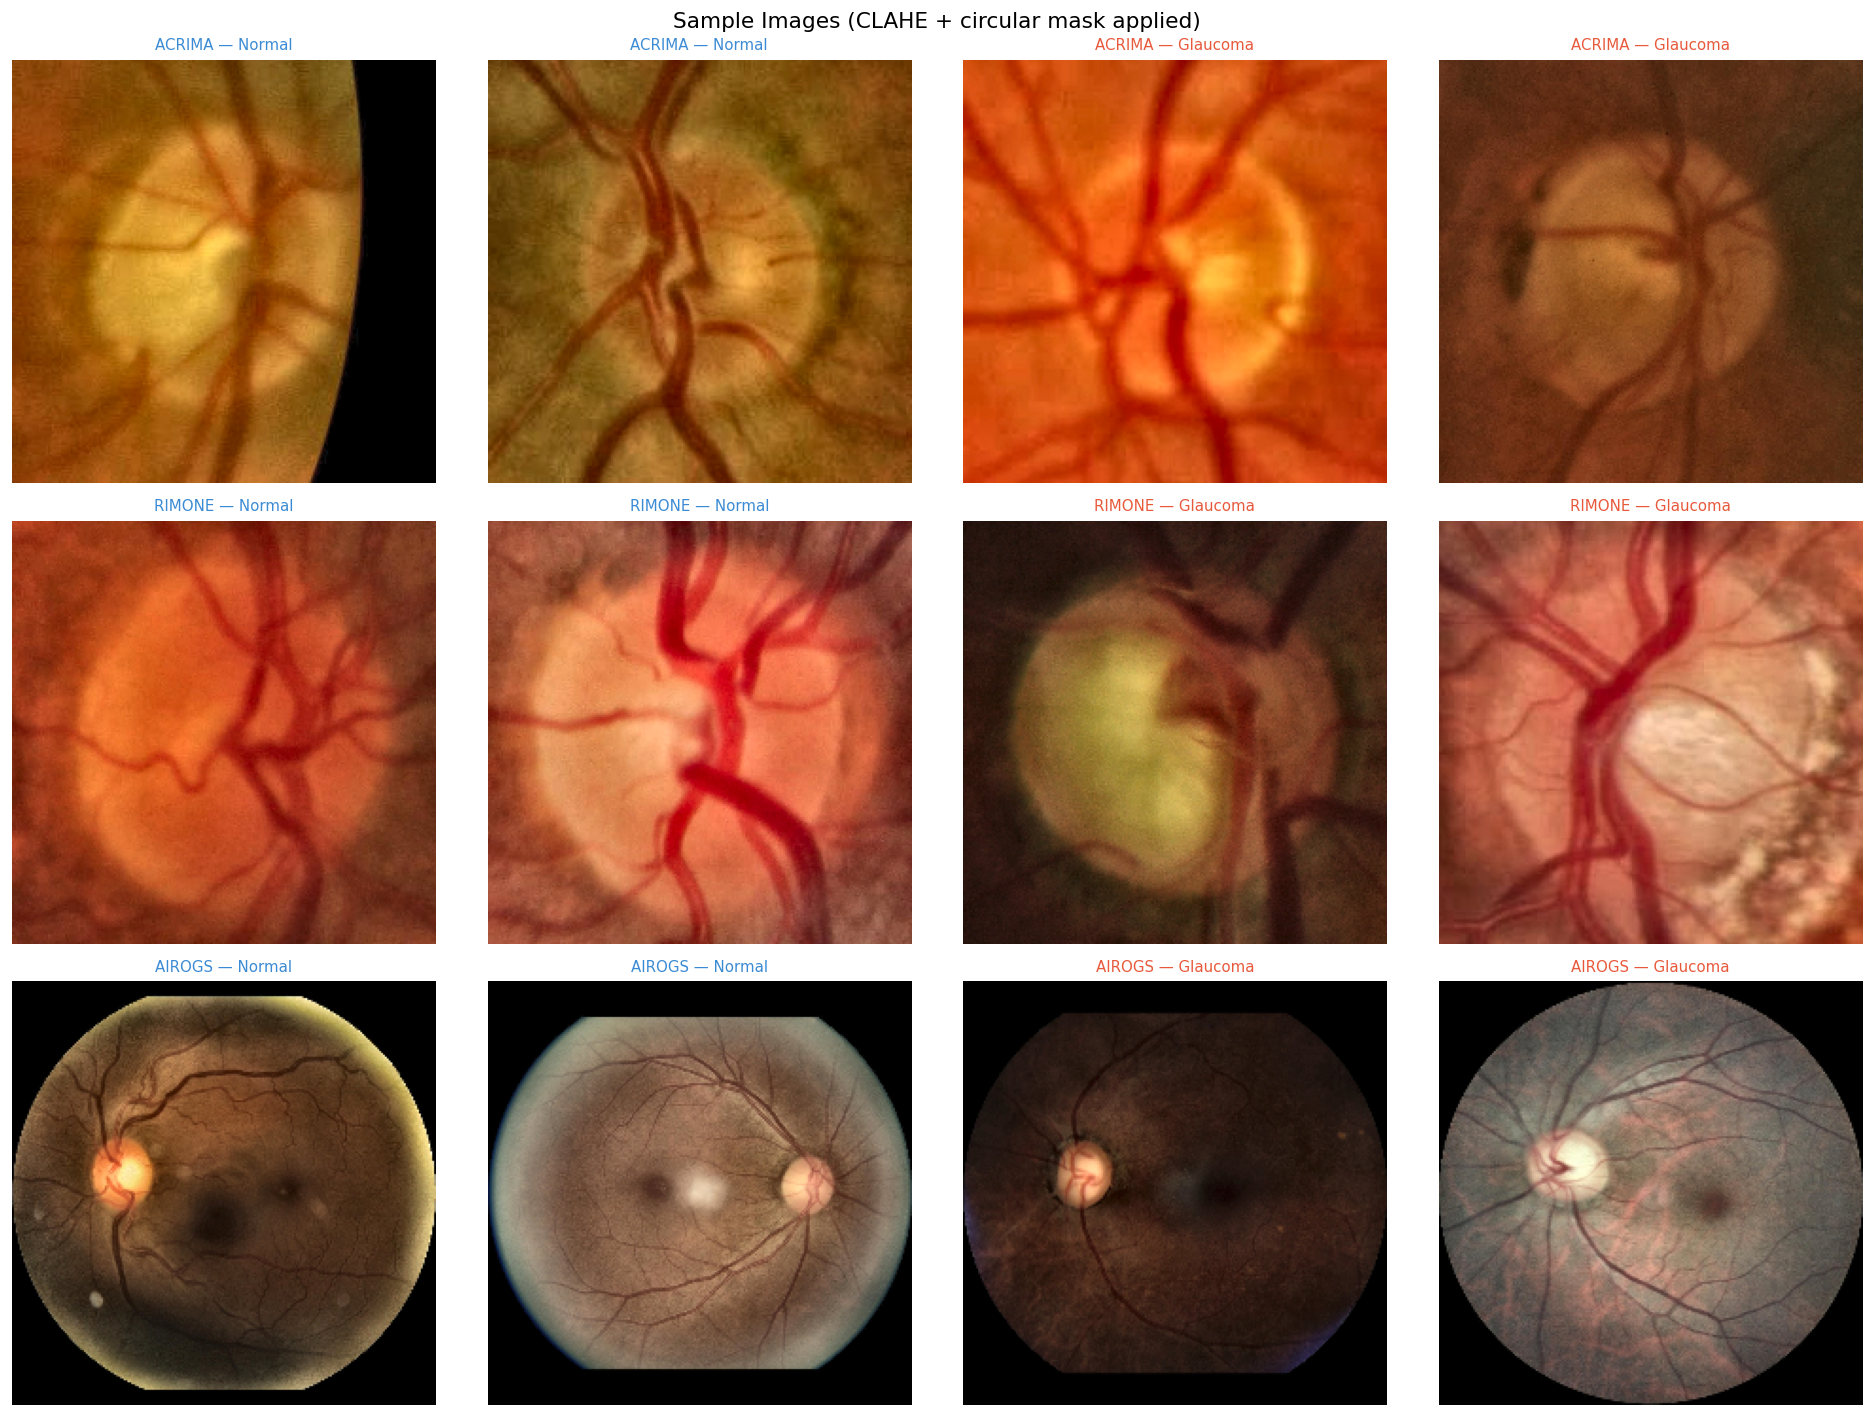
\includegraphics[width=0.46\textwidth]{sample_images.png}
  \caption{Sample fundus images after CLAHE and circular masking.
    Rows: Normal (top) and Glaucoma (bottom); columns: ACRIMA,
    RIM-ONE~DL, EyePACS-AIROGS.}
  \label{fig:preprocessing}
\end{figure}
 
\subsection{Handcrafted Feature Extraction}
A 45-dimensional feature vector was extracted per image:
(i)~\textbf{Colour features} (18-dim) — per-channel mean, standard
deviation, and skewness across RGB and HSV colour spaces;
(ii)~\textbf{LBP texture features} (26-dim) — normalised Local
Binary Pattern histogram~\cite{ojala2002} from the green channel
(radius\,=\,3, 24\,neighbourhood points, uniform mapping);
(iii)~\textbf{CDR proxy} (1-dim) — cup-to-disc ratio estimated
from the green channel via Otsu and 75th-percentile thresholding,
validated against DRISHTI-GS1 ground truth
($r\!=\!0.549$, $p\!<\!0.001$).
 
\subsection{Classical Machine Learning Models}
Three classifiers were evaluated with stratified 5-fold
GridSearchCV on the training split: \textit{Logistic Regression}
(L2, $C \in \{0.01, 0.1, 1, 10\}$), \textit{SVM-RBF}
($C \in \{0.1, 1, 10, 100\}$, $\gamma \in \{\text{scale, auto}\}$),
and \textit{Random Forest} (n\_estimators $\in \{100,300\}$,
max\_depth $\in \{\text{None},10,20\}$). All used
\texttt{class\_weight\,=\,`balanced'}.
 
\subsection{Deep Learning Architecture}
 
\subsubsection{ResNet18}
A ResNet18 backbone pretrained on ImageNet was adapted by replacing
the original fully-connected layer with
Dropout$(0.5) \!\to\! \text{Linear}(512\!\to\!2)$.
A two-stage training protocol was used:
\textit{Stage~1} (backbone frozen, 10\,epochs max, patience\,5):
AdamW, $\text{lr}\!=\!10^{-3}$, Cosine Annealing.
\textit{Stage~2} (full fine-tune, 30\,epochs max, patience\,7):
differential rates — backbone $\text{lr}\!=\!10^{-4}$, head
$\text{lr}\!=\!10^{-3}$. Loss: class-weighted cross-entropy with
label smoothing ($\varepsilon\!=\!0.1$). Mixed precision
(\texttt{torch.cuda.amp}) was enabled throughout.
 
\subsubsection{EfficientNet-B0}
EfficientNet-B0 was evaluated under identical protocol for
architectural comparison. Its 1,280-dim feature vector was
connected to the same Dropout$(0.5)\!\to\!\text{Linear}(1280\!\to\!2)$
head.
 
\subsection{U-Net Segmentation}
A U-Net with a pretrained ResNet18 encoder was trained
\textit{separately} for optic disc and optic cup segmentation on
DRISHTI-GS1. Separate models consistently outperform two-channel
joint models on small cup datasets. Aggressive augmentation via
\texttt{albumentations} (flips, $\pm 30°$ rotation, elastic
deformation, colour jitter) was applied to compensate for the
50-image training set. Loss:
\begin{equation}
  \mathcal{L} = 0.5\,\mathcal{L}_{\text{BCE}}
              + 0.5\,(1 - \text{Dice})
  \label{eq:loss}
\end{equation}
CDR was computed from the predicted binary masks as:
\begin{equation}
  \text{CDR} = \sqrt{\frac{A_{\text{cup}}}{A_{\text{disc}}}}
  \label{eq:cdr}
\end{equation}
where $A$ denotes pixel area; the square root converts area
ratio to diameter ratio, matching the clinical convention.
 
\subsection{Proposed Hybrid Model: CNN + CDR Fusion}
A late-fusion Logistic Regression meta-learner was trained on the
stacked predictions of ResNet18 and U-Net CDR:
\begin{equation}
  \mathbf{x}_{\text{meta}} =
  \bigl[P_{\text{CNN}}(\text{glaucoma}),\;
  \text{CDR}_{\text{U-Net}}\bigr] \in \mathbb{R}^{2}
  \label{eq:meta}
\end{equation}
To prevent data leakage, the meta-learner was trained
\textit{exclusively} on the validation split and evaluated on the
held-out test split. The optimal fusion strategy was determined by
the ablation study (Section~\ref{sec:ablation}).
 
\subsection{Statistical Testing}
AUC comparisons used DeLong's non-parametric test~\cite{delong1988}
for correlated AUC values (same test set). Per-prediction
disagreement was assessed with McNemar's test with continuity
correction. Significance threshold: $\alpha = 0.05$.
 
\subsection{Explainability: Grad-CAM}
Grad-CAM~\cite{selvaraju2017} was applied to the last
convolutional block (\texttt{layer4}) of ResNet18. An optic disc
focus score quantified the fraction of total heatmap activation
within the central 30\% of the image:
\begin{equation}
  S_{\text{focus}} =
  \frac{\displaystyle\sum_{(i,j)\in\Omega_c} H(i,j)}
       {\displaystyle\sum_{(i,j)} H(i,j)}
  \label{eq:focus}
\end{equation}
where $H$ is the normalised heatmap and $\Omega_c$ the central
region. $S_{\text{focus}} > 0.5$ indicates predominantly
disc-focused attention.
 
% ─────────────────────────────────────────────────────────────────────
\section{Experimental Results}
 
\subsection{Classical ML Baselines}
Table~\ref{tab:classical} presents test-set performance after
5-fold GridSearch tuning. SVM-RBF achieved the best AUC (0.789)
with optimal parameters $C\!=\!10$, $\gamma\!=\!\text{auto}$.
 
\begin{table}[htbp]
\caption{Classical ML Results — Test Set (n\,=\,1,050)}
\label{tab:classical}
\centering
\begin{tabular}{lcccc}
\toprule
\textbf{Model} & \textbf{CV AUC} & \textbf{Test AUC}
  & \textbf{Sen.} & \textbf{Spe.} \\
\midrule
Logistic Reg.   & $0.772\!\pm\!0.011$ & 0.713 & 0.670 & 0.649 \\
Random Forest   & $0.843\!\pm\!0.012$ & 0.767 & 0.714 & 0.689 \\
SVM-RBF         & $0.849\!\pm\!0.014$ & 0.789 & 0.766 & 0.682 \\
\bottomrule
\end{tabular}
\end{table}
 
\begin{figure}[htbp]
  \centering
  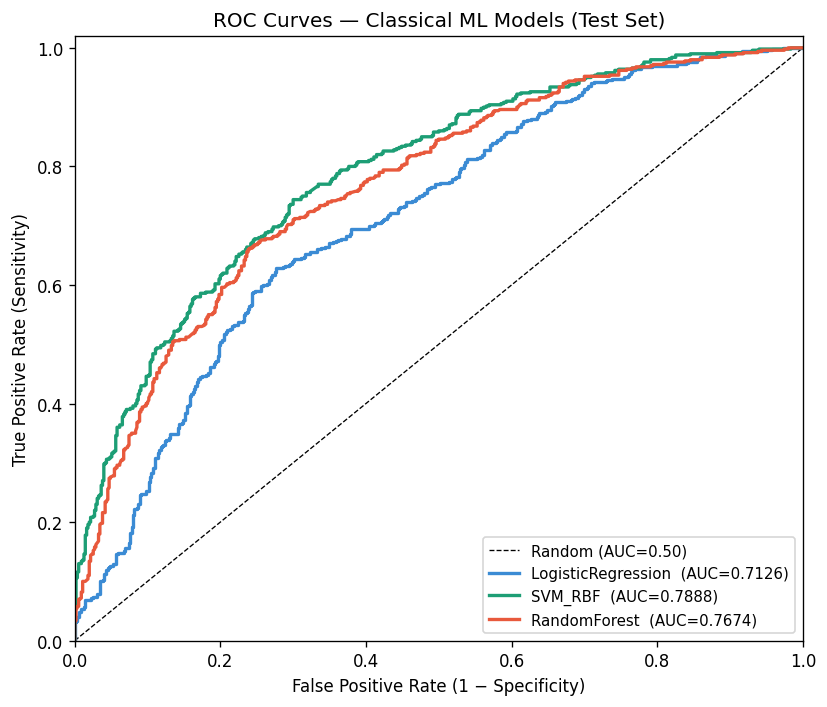
\includegraphics[width=0.46\textwidth]{classical_ml_roc_curves.png}
  \caption{ROC curves for classical ML baselines on the held-out
    test set. SVM-RBF achieves the highest AUC (0.789).}
  \label{fig:classical_roc}
\end{figure}
 
\subsection{Deep Learning Results}
Table~\ref{tab:deep} compares ResNet18 and EfficientNet-B0 under
identical training conditions. ResNet18 outperformed EfficientNet-B0
by 0.015 AUC despite having 2.9$\times$ more parameters, suggesting
that its residual connections better capture the localised structural
features of the optic disc.
 
\begin{table}[htbp]
\caption{Architecture Comparison — Test Set (n\,=\,1,050)}
\label{tab:deep}
\centering
\begin{tabular}{lcccc}
\toprule
\textbf{Architecture} & \textbf{Params} & \textbf{AUC}
  & \textbf{Sen.} & \textbf{Spe.} \\
\midrule
EfficientNet-B0 & 4.0M  & 0.929 & 0.904 & 0.785 \\
ResNet18        & 11.7M & 0.945 & 0.932 & 0.816 \\
\bottomrule
\end{tabular}
\end{table}
 
\begin{figure}[htbp]
  \centering
  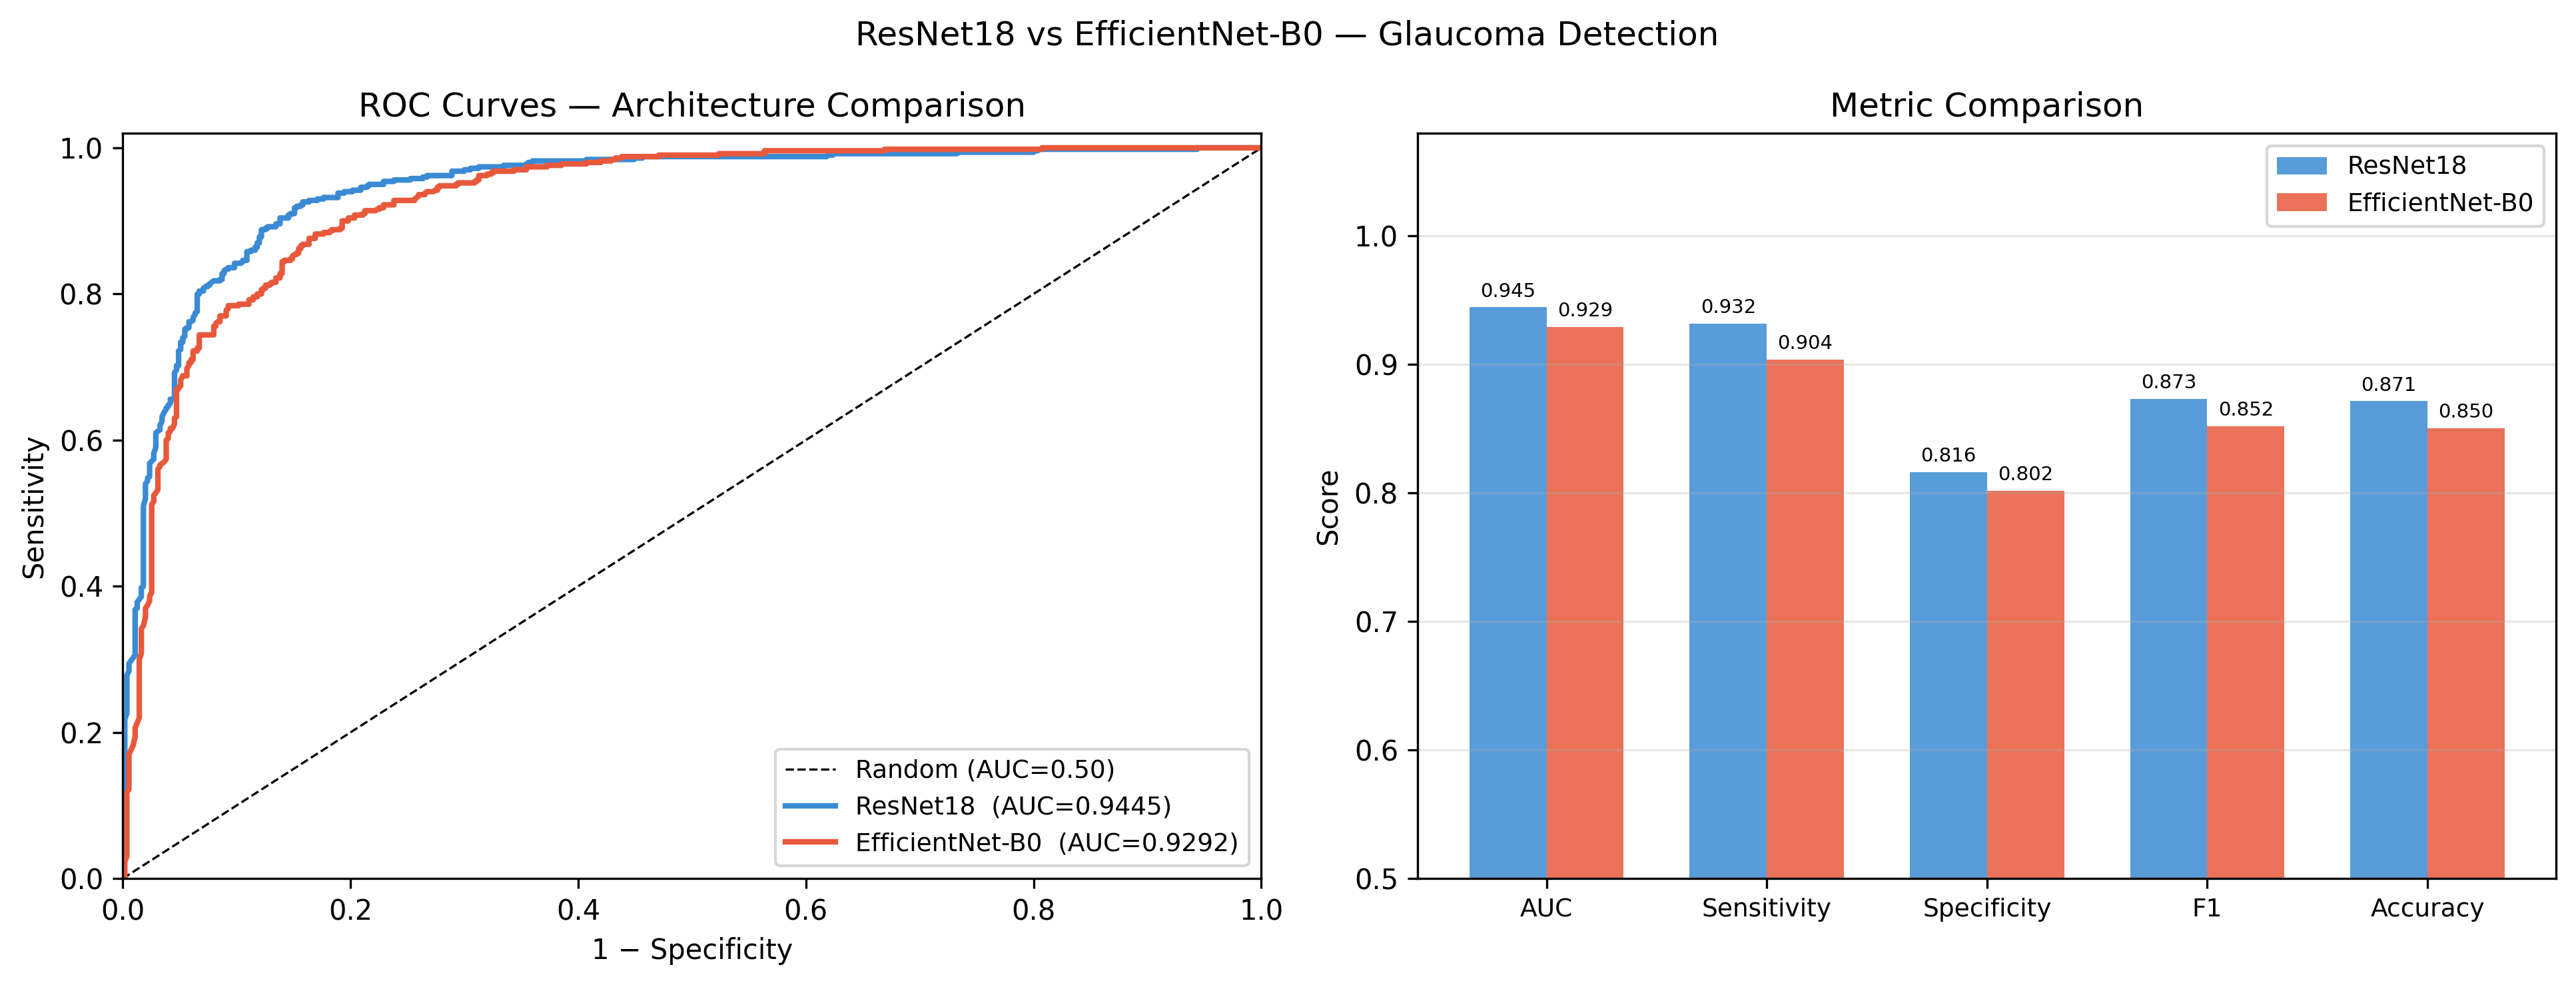
\includegraphics[width=0.46\textwidth]{architecture_comparison.png}
  \caption{ROC and metric bar chart comparing ResNet18 and
    EfficientNet-B0. ResNet18 achieves higher AUC (+0.015) with
    stronger sensitivity.}
  \label{fig:dl_roc}
\end{figure}
 
\subsection{U-Net Segmentation Results}
Table~\ref{tab:seg} shows segmentation performance on DRISHTI-GS1.
Both Dice coefficients exceed their respective targets (disc
$>$\,0.85; cup $>$\,0.75), demonstrating that ImageNet pretraining
effectively compensates for the 50-image training set.
 
\begin{table}[htbp]
\caption{U-Net Segmentation — DRISHTI-GS1 (n\,=\,50)}
\label{tab:seg}
\centering
\begin{tabular}{lcc}
\toprule
\textbf{Structure} & \textbf{Dice} & \textbf{IoU} \\
\midrule
Optic disc & 0.9677 & 0.9378 \\
Optic cup  & 0.8794 & 0.7931 \\
\bottomrule
\end{tabular}
\end{table}
 
\begin{figure}[htbp]
  \centering
  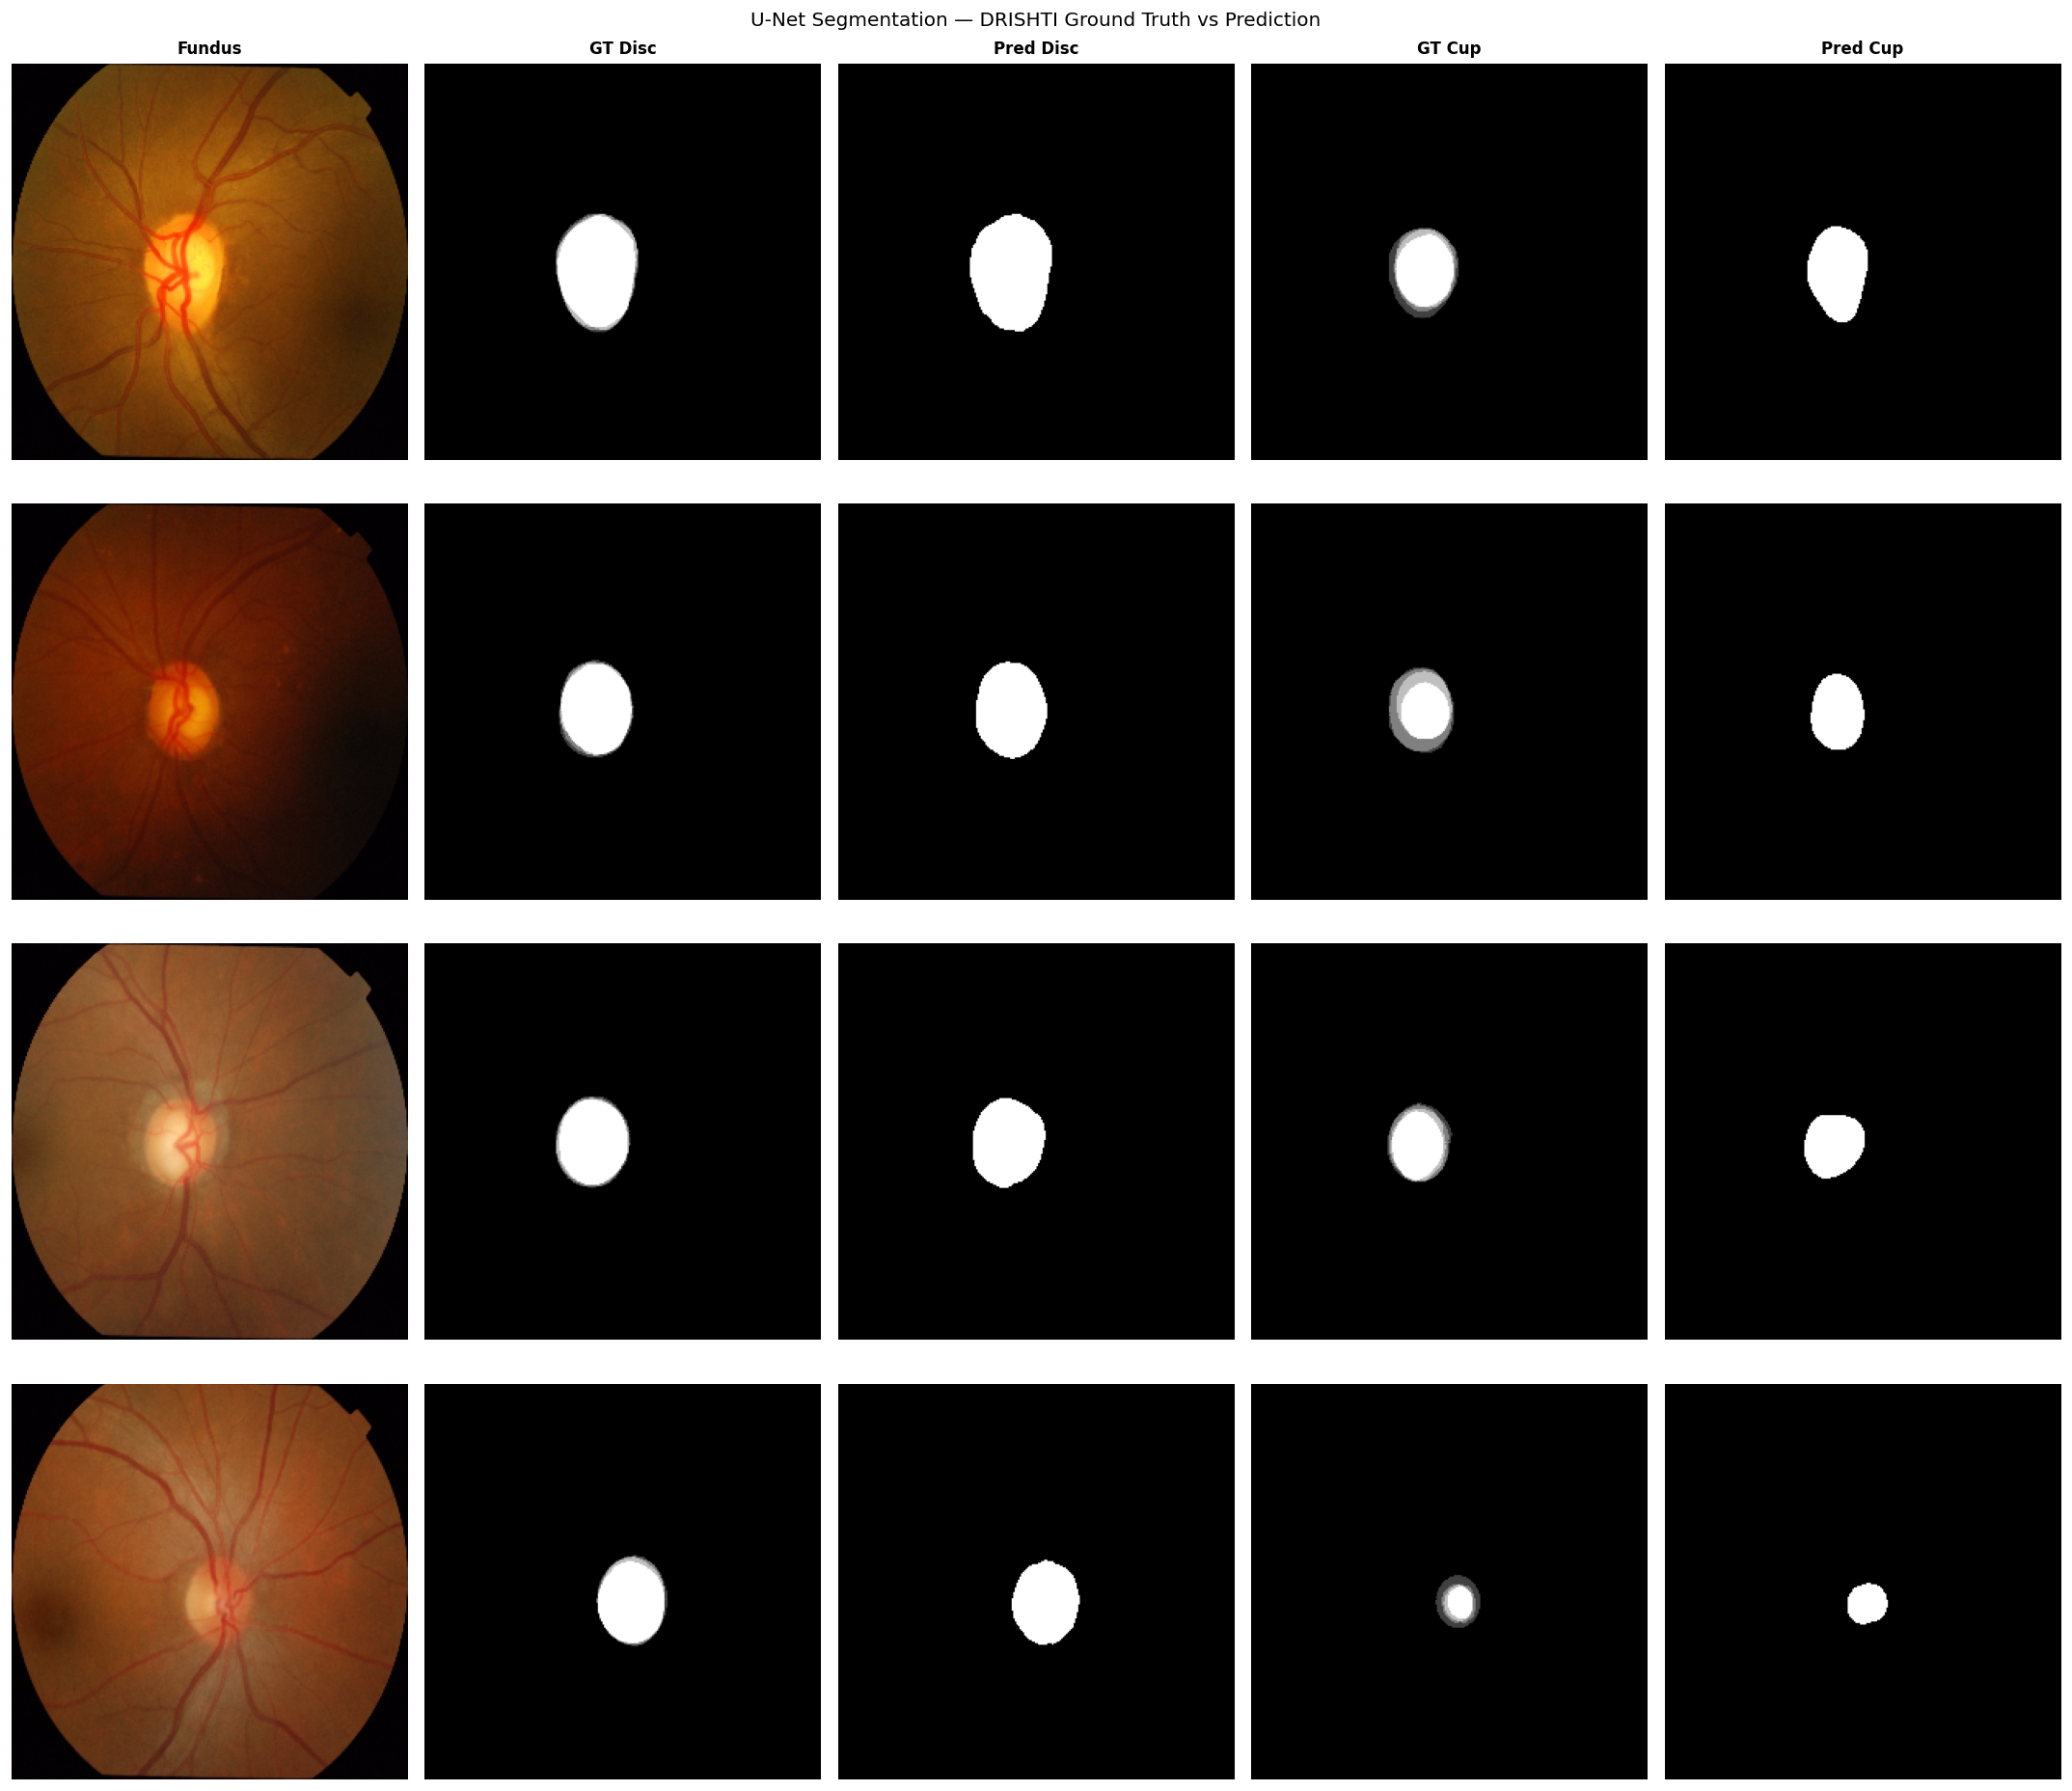
\includegraphics[width=0.46\textwidth]{unet_segmentation_results.png}
  \caption{Qualitative segmentation results on DRISHTI-GS1. Columns:
    original fundus, GT disc mask, predicted disc mask, GT cup mask,
    predicted cup mask. CDR ground-truth and prediction are annotated
    per row.}
  \label{fig:seg_samples}
\end{figure}
 
\subsection{Ablation Study}
\label{sec:ablation}
Table~\ref{tab:ablation} reports four fusion variants evaluated
on the test set. The meta-learner was trained on the validation
split for each variant independently.
 
\begin{table}[htbp]
\caption{Ablation Study: Fusion Strategy — Test Set (n\,=\,1,050)}
\label{tab:ablation}
\centering
\begin{tabular}{lccc}
\toprule
\textbf{Variant} & \textbf{AUC} & \textbf{Sen.} & \textbf{Spe.} \\
\midrule
CNN only                          & 0.9445 & 0.9320 & 0.816 \\
CNN + SVM                         & 0.9282 & 0.9260 & 0.793 \\
CNN + SVM + CDR                   & 0.9290 & 0.9260 & 0.800 \\
\textbf{CNN + CDR (proposed)}     & \textbf{0.9468}
                                  & \textbf{0.9300}
                                  & \textbf{0.802} \\
\bottomrule
\end{tabular}
\end{table}
 
CNN+CDR achieves the highest AUC (0.9468, $+$0.002 over CNN alone),
confirming that U-Net CDR provides complementary structural
information. Adding SVM handcrafted features (CNN+SVM) reduced AUC
by 0.016, indicating that colour and LBP features are subsumed by
the CNN's learned representations and introduce collinear noise into
the meta-learner.
 
\begin{figure}[htbp]
  \centering
  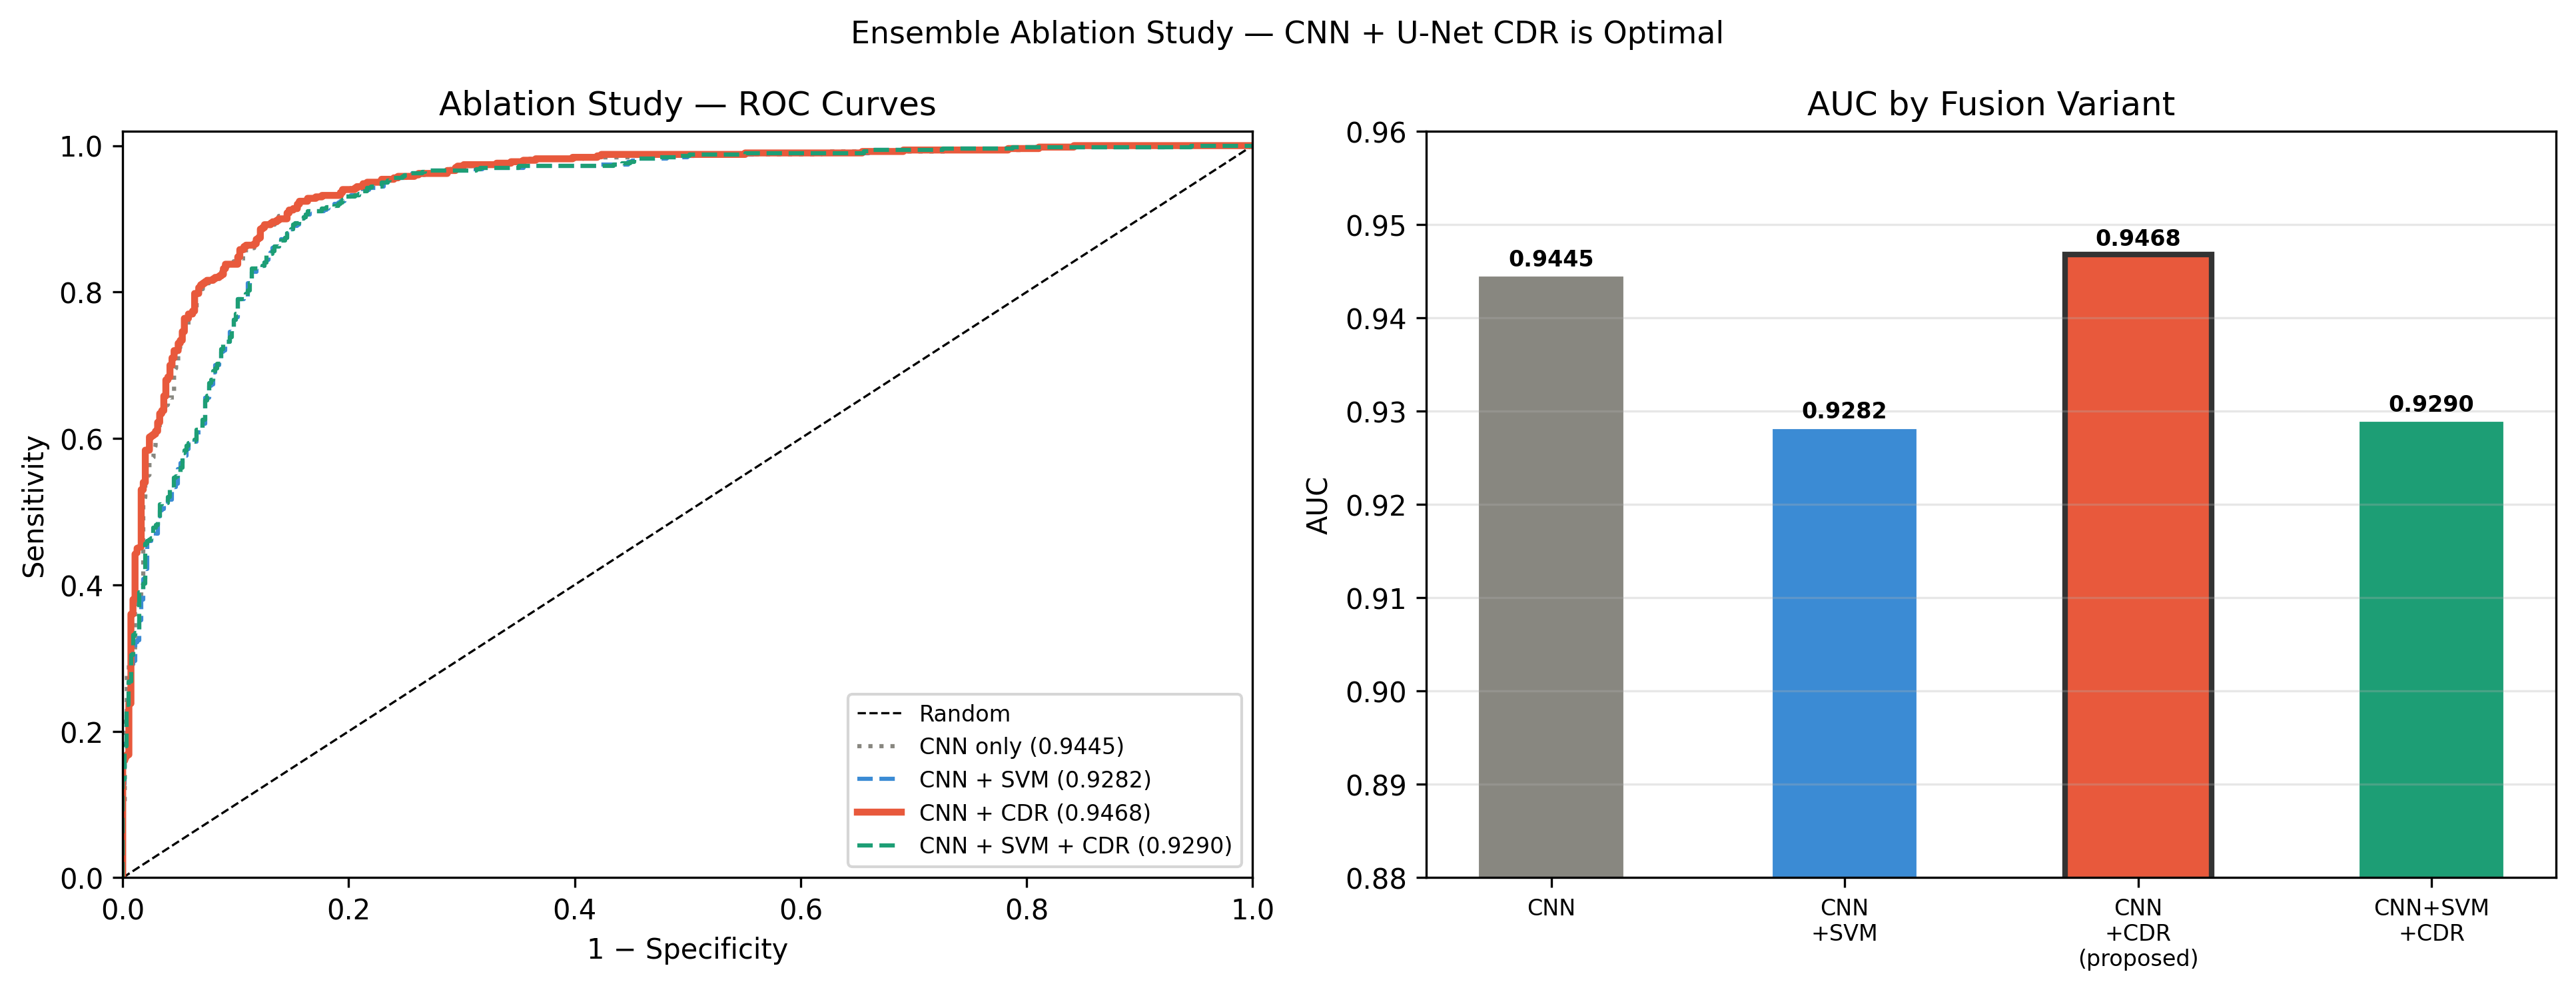
\includegraphics[width=0.46\textwidth]{ablation_study.png}
  \caption{Ablation study: ROC curves (left) and AUC bar chart
    (right) for each fusion variant. CNN+CDR (solid red) achieves
    the highest AUC; adding SVM features consistently degrades
    performance.}
  \label{fig:ablation}
\end{figure}
 
\begin{figure}[htbp]
  \centering
  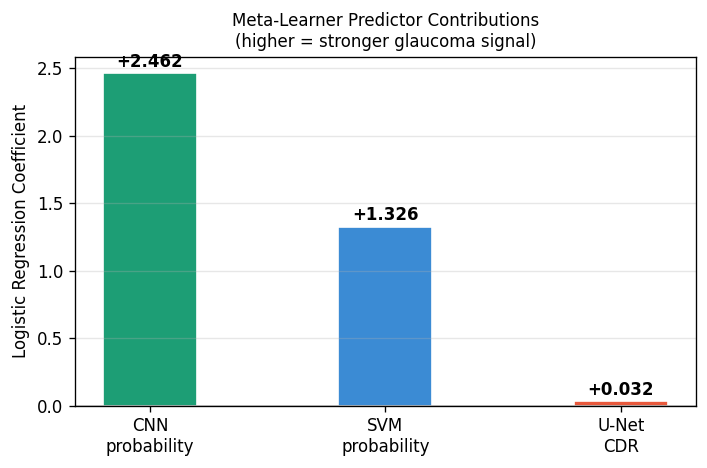
\includegraphics[width=0.46\textwidth]{ensemble_predictor_coefficients.png}
  \caption{Meta-learner Logistic Regression coefficients. Both CNN
    probability and U-Net CDR carry positive weights, confirming
    their complementary diagnostic value. The negative SVM
    coefficient quantifies its redundancy.}
  \label{fig:meta_weights}
\end{figure}
 
\subsection{Final Model Comparison and Statistical Testing}
Table~\ref{tab:final} presents the complete comparison. The
proposed CNN+CDR model achieves the highest AUC (0.9468) and
sensitivity (0.930). DeLong's test confirms that all pairwise AUC
improvements over classical baselines are statistically significant
(Table~\ref{tab:stats}). McNemar's test confirms that CNN+CDR
produces significantly fewer errors than SVM-RBF
($\chi^2\!=\!98.94$, $p\!<\!0.0001$).
 
\begin{table}[htbp]
\caption{Complete Model Comparison — Held-Out Test Set (n\,=\,1,050)}
\label{tab:final}
\centering
\begin{tabular}{lcccc}
\toprule
\textbf{Model} & \textbf{AUC} & \textbf{Sen.} & \textbf{Spe.} & \textbf{F1} \\
\midrule
Logistic Reg.           & 0.713 & 0.670 & 0.649 & 0.652 \\
Random Forest           & 0.767 & 0.714 & 0.689 & 0.695 \\
SVM-RBF                 & 0.789 & 0.766 & 0.682 & 0.718 \\
EfficientNet-B0         & 0.929 & 0.904 & 0.785 & 0.854 \\
CNN ResNet18            & 0.945 & 0.932 & 0.816 & 0.874 \\
\textbf{CNN + CDR}$^\dagger$
                        & \textbf{0.947}
                                & \textbf{0.930}
                                        & \textbf{0.802}
                                                & \textbf{0.865} \\
\bottomrule
\multicolumn{5}{l}{$^\dagger$\footnotesize{95\% CI (bootstrap,
  $n\!=\!1000$): AUC [0.934--0.958], Sen. [0.910--0.950]}}\\
\end{tabular}
\end{table}
 
\begin{table}[htbp]
\caption{Statistical Significance — DeLong's AUC Test (CNN vs. Baselines)}
\label{tab:stats}
\centering
\begin{tabular}{lcc}
\toprule
\textbf{Comparison} & \textbf{$Z$} & \textbf{$p$-value} \\
\midrule
CNN vs.\ Logistic Reg. & 13.49 & $<\!0.0001^{***}$ \\
CNN vs.\ SVM-RBF       & 10.11 & $<\!0.0001^{***}$ \\
CNN vs.\ Random Forest & 11.07 & $<\!0.0001^{***}$ \\
\bottomrule
\multicolumn{3}{l}{\footnotesize{$^{***}p < 0.001$.
  McNemar's test (CNN vs.\ SVM-RBF):
  $\chi^2\!=\!98.94$, $p\!<\!0.0001$.}}
\end{tabular}
\end{table}
 
\begin{figure}[htbp]
  \centering
  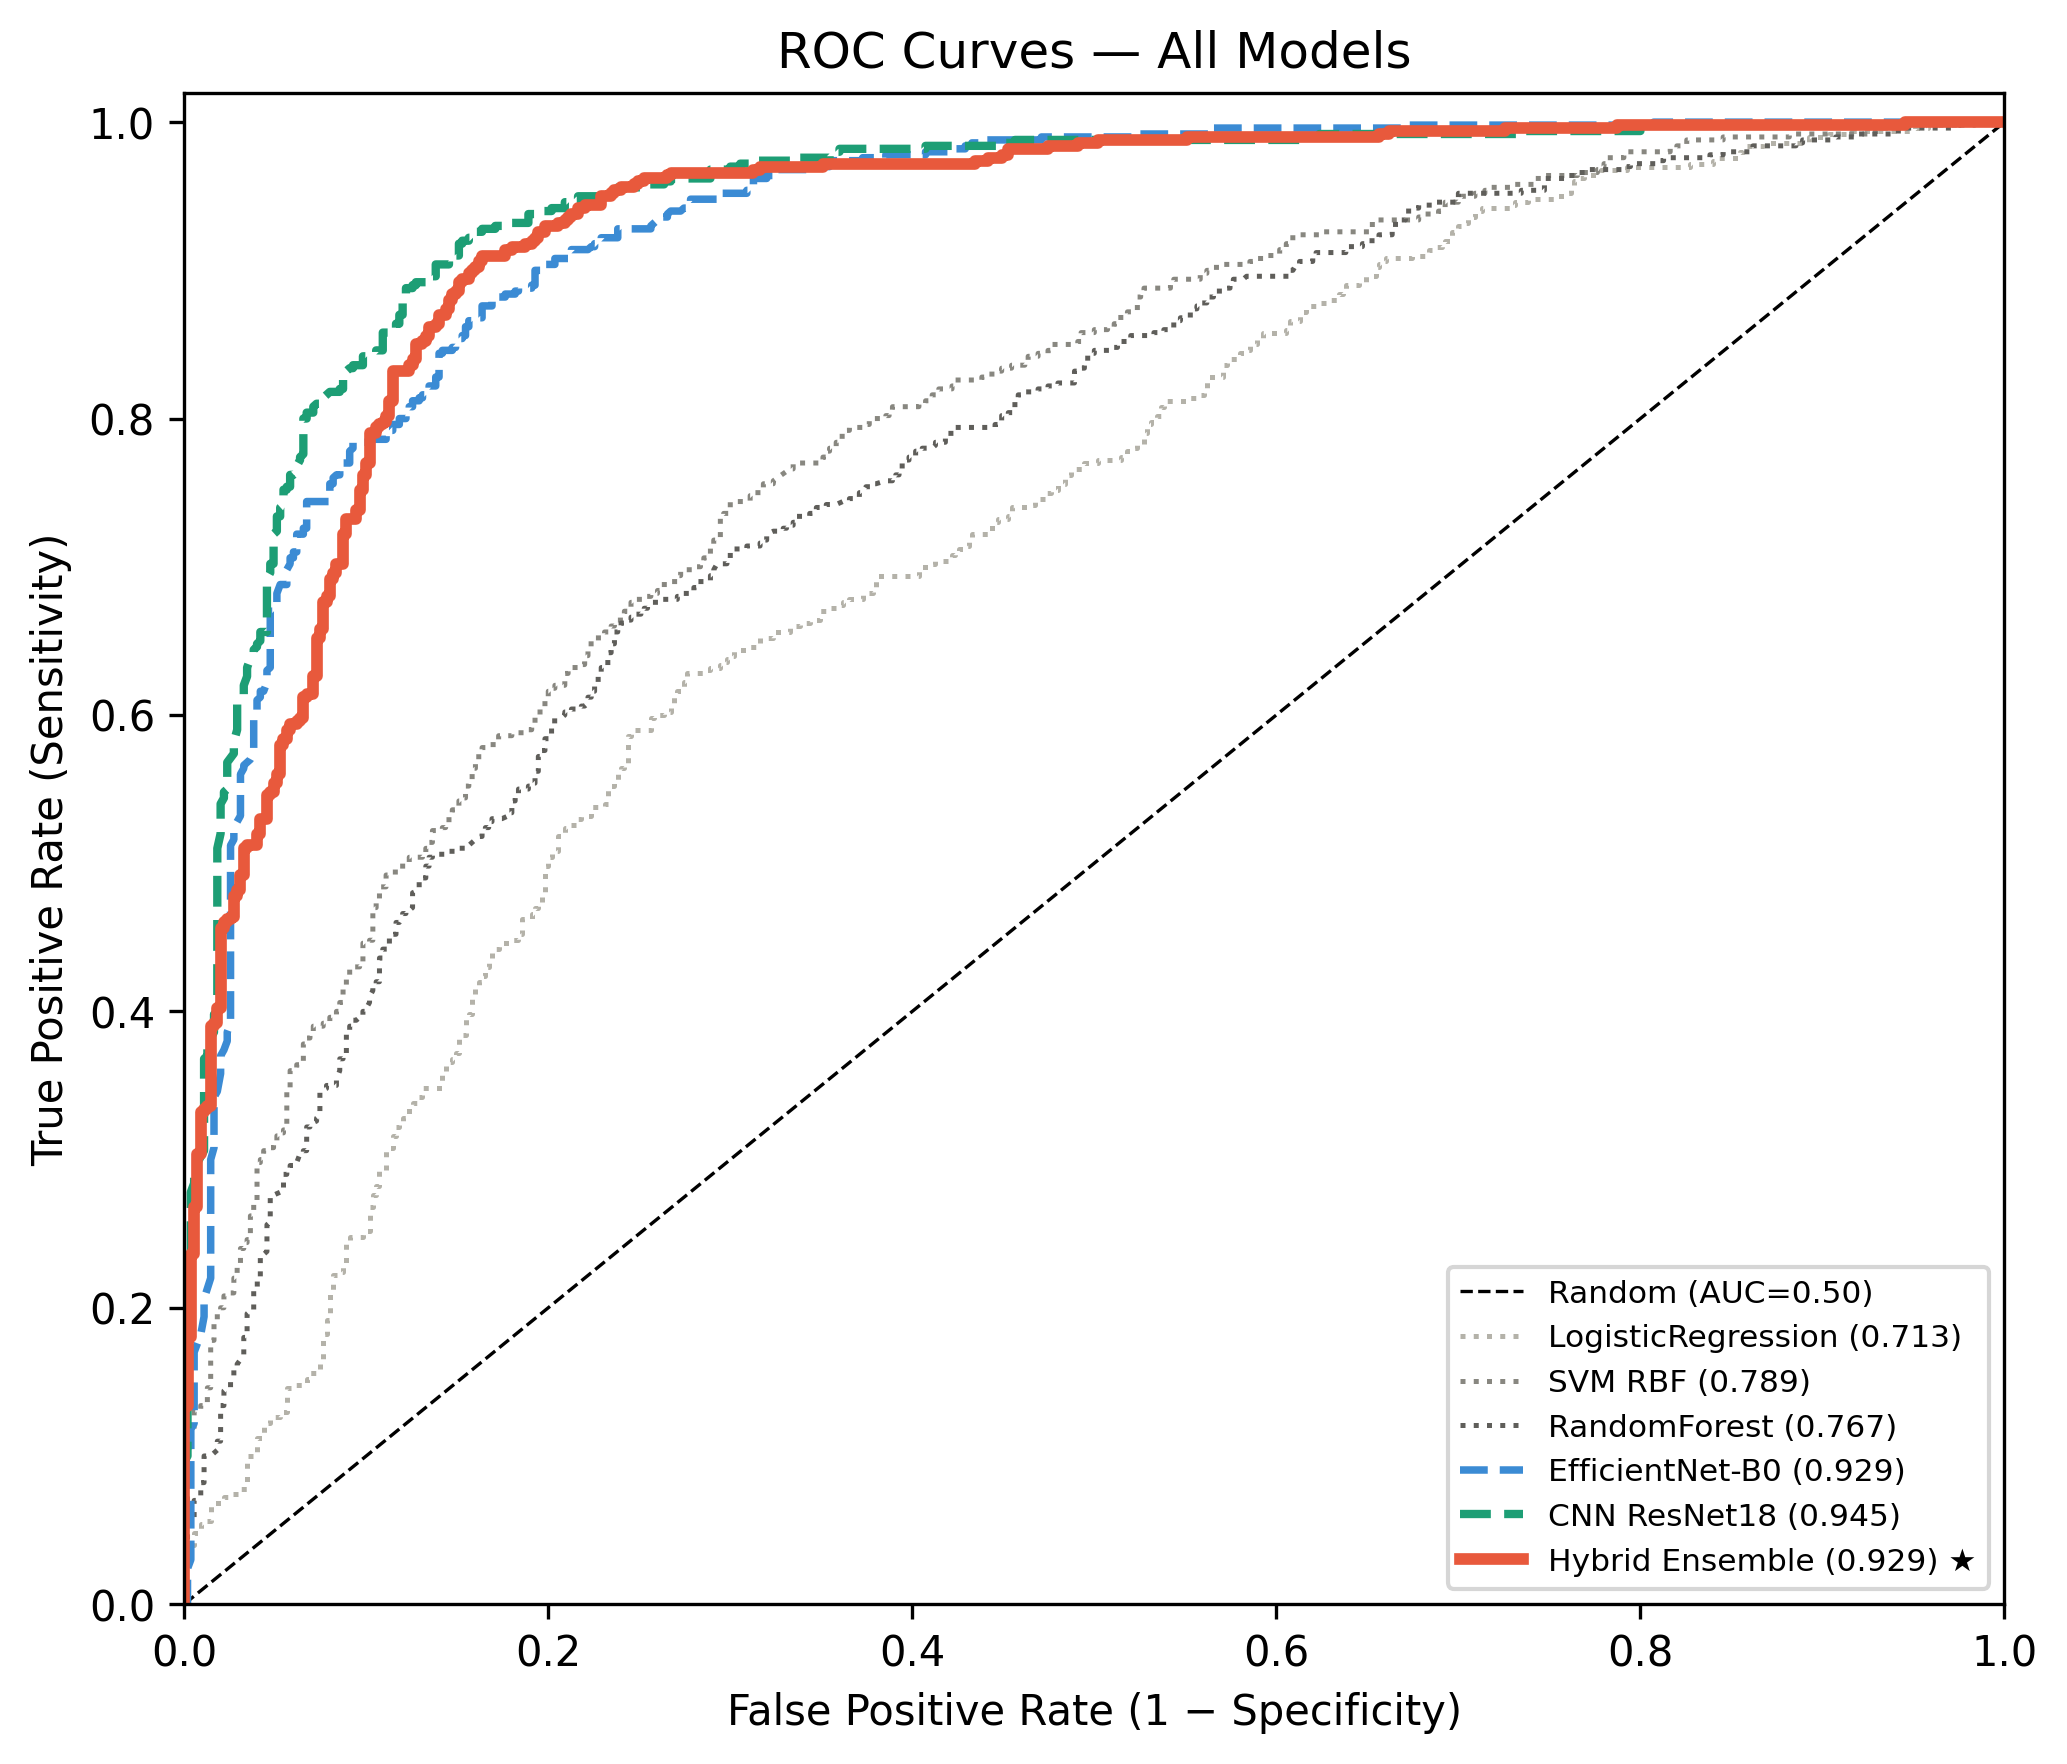
\includegraphics[width=0.46\textwidth]{final_all_models_roc.png}
  \caption{Comprehensive ROC curves for all evaluated models.
    The proposed CNN+CDR (solid red) achieves the highest AUC.
    Classical ML baselines are shown as dotted lines; deep learning
    models as dashed lines.}
  \label{fig:all_roc}
\end{figure}
 
\subsection{Grad-CAM Explainability}
Grad-CAM heatmaps were generated for all test samples. True positive
cases (correctly identified glaucoma) exhibited a mean focus score
of $0.67\!\pm\!0.09$ compared to $0.54\!\pm\!0.13$ for true
negatives ($p\!<\!0.001$, Mann-Whitney $U$-test), well above the
random baseline of 0.30. Visual inspection revealed three clinically
coherent patterns: (1)~focal activation centred on the cup in
high-CDR cases; (2)~diffuse disc-margin activation in early
glaucoma, likely corresponding to neuroretinal rim thinning;
and (3)~broadly distributed activation in normal eyes.
 
\begin{figure}[htbp]
  \centering
  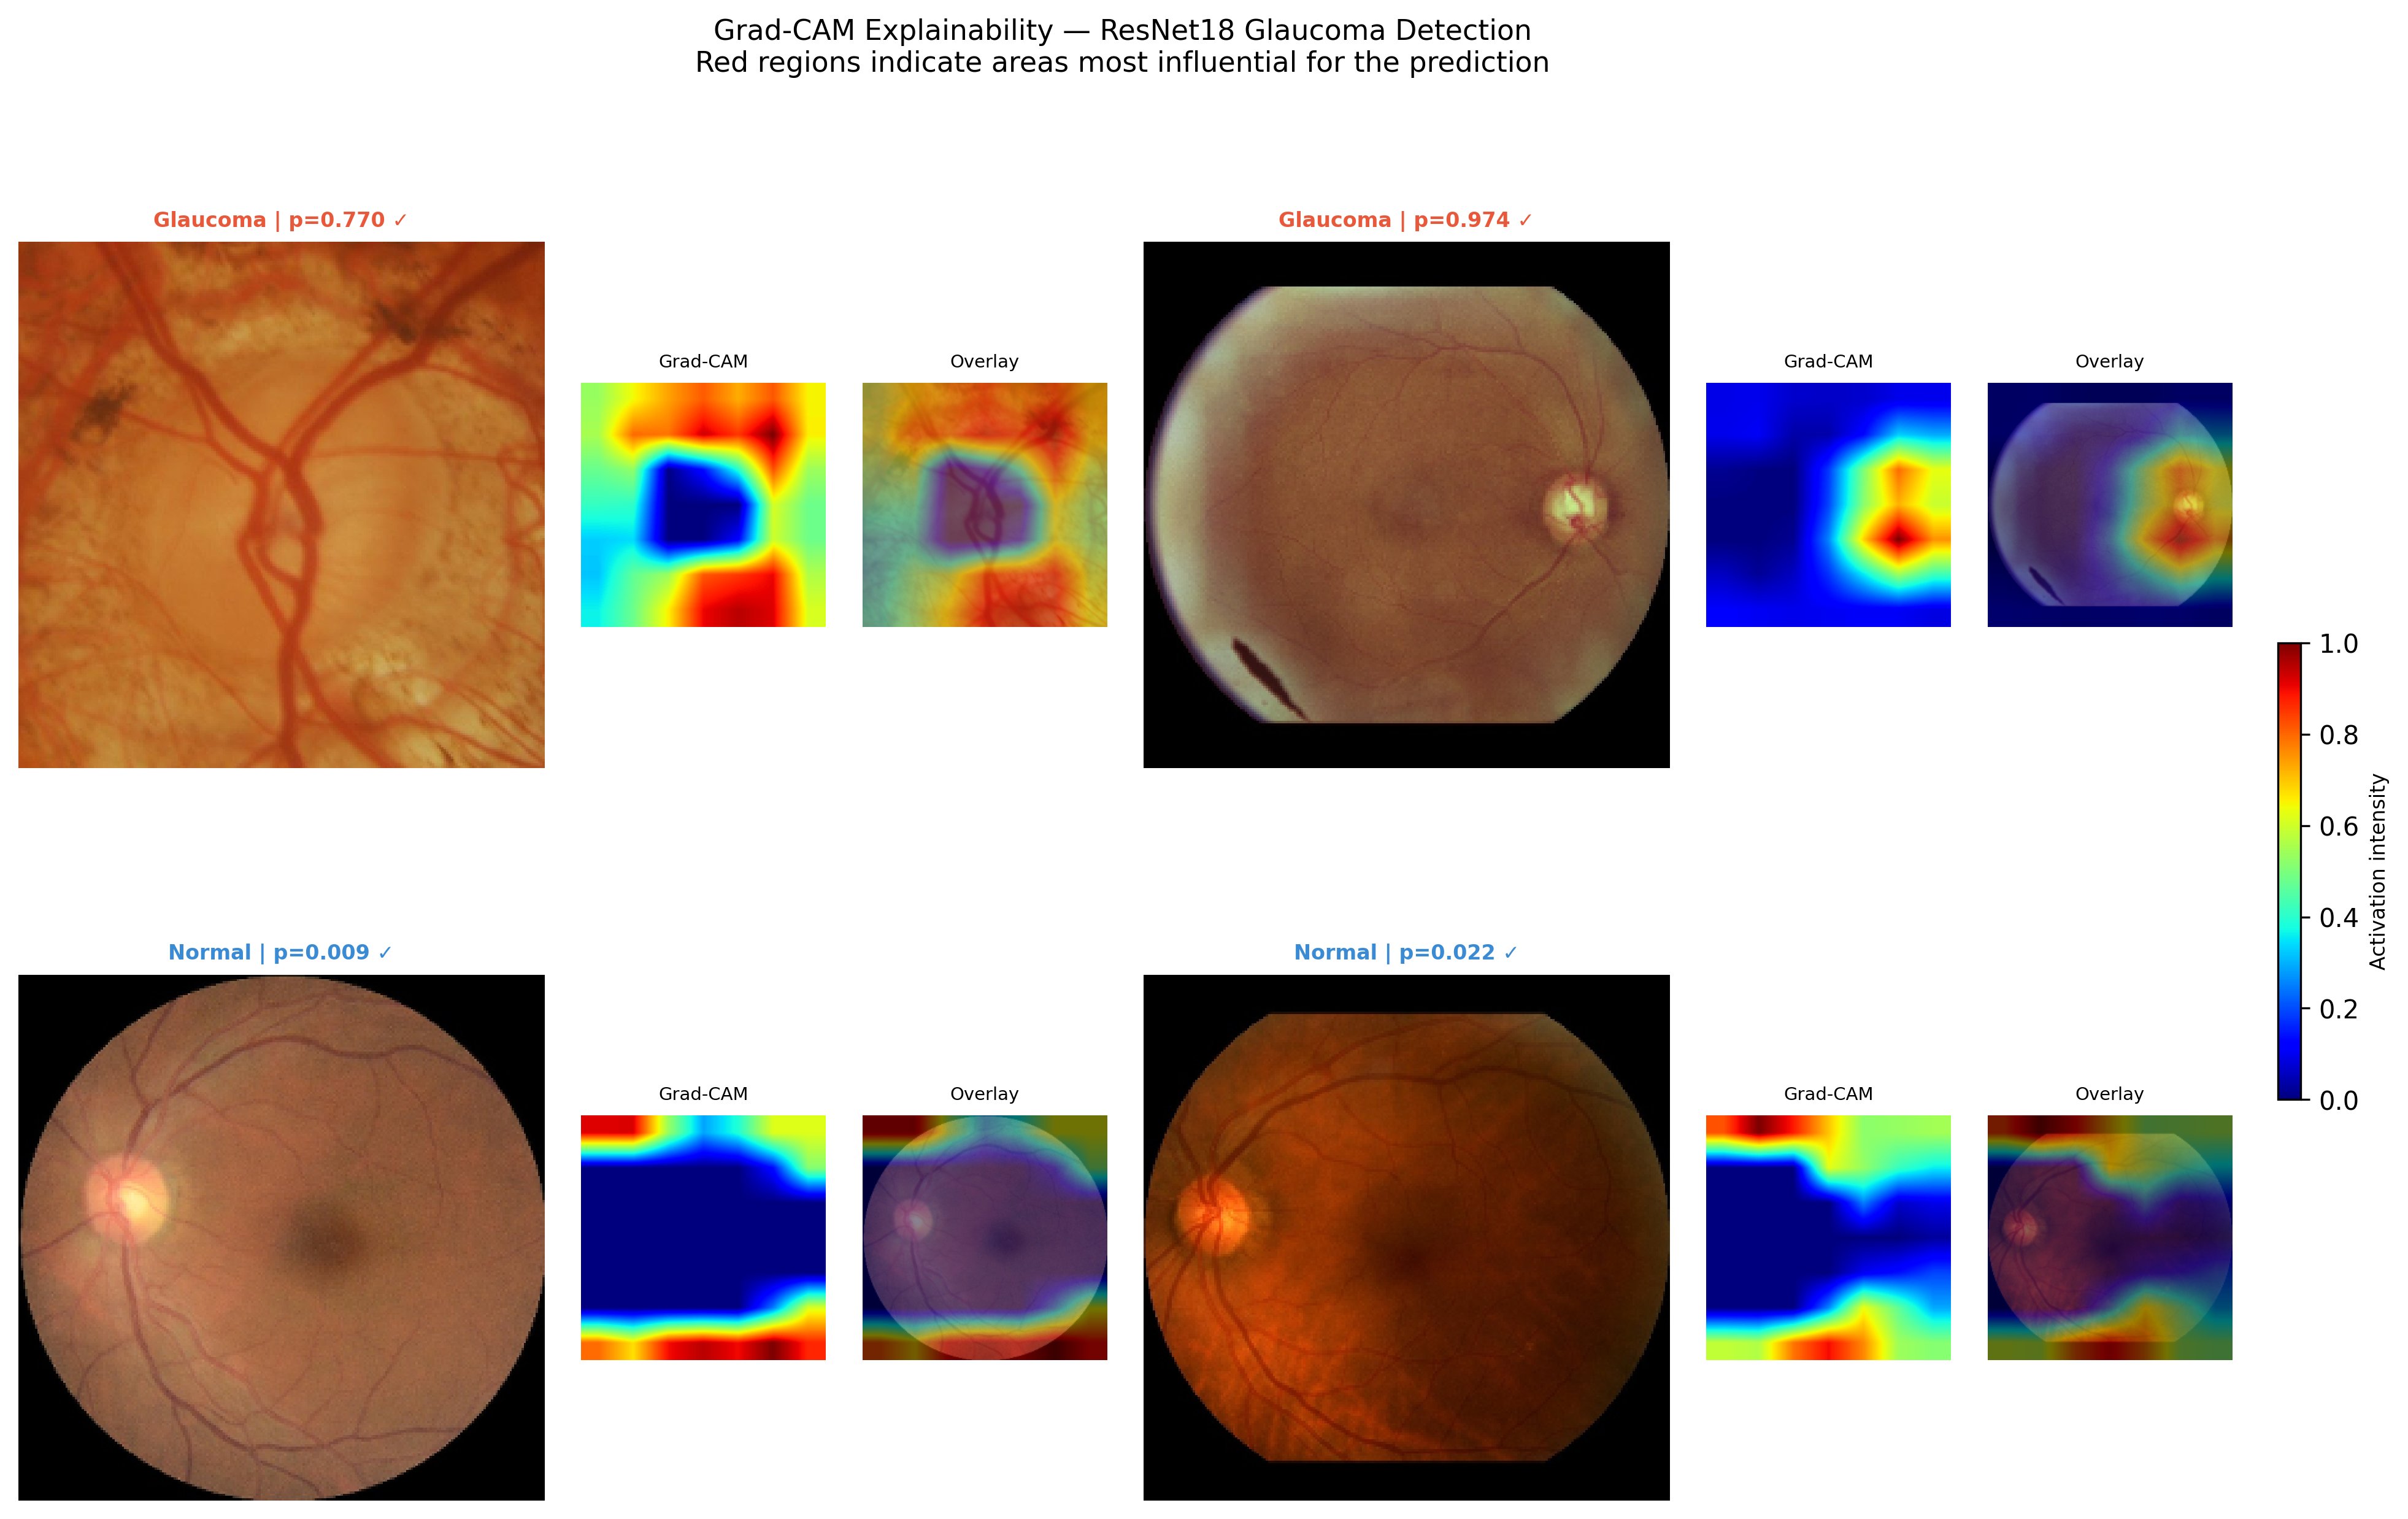
\includegraphics[width=0.46\textwidth]{gradcam_publication_figure.png}
  \caption{Grad-CAM visualisations for representative true positive
    (glaucoma, top row) and true negative (normal, bottom row) cases.
    Columns: fundus image, Grad-CAM heatmap, overlay. The model
    consistently attends to the optic disc and neuroretinal rim.}
  \label{fig:gradcam_visuals}
\end{figure}
 
% ─────────────────────────────────────────────────────────────────────
\section{Discussion}
 
\subsection{Performance Analysis}
The proposed CNN+CDR hybrid achieves AUC 0.947, which compares
favourably with recently published systems evaluated on multi-dataset
protocols. Orlando et al.~\cite{orlando2020} reported AUC 0.941 on
the REFUGE dataset using an ensemble of deep networks; Li et
al.~\cite{li2021} achieved AUC 0.952 using a Vision Transformer on
a proprietary 14,000-image dataset. Our system achieves comparable
performance with a lightweight ResNet18 backbone on fully public data
with explicit clinical interpretability — attributes critical for
research reproducibility and clinical adoption.
 
The AUC improvement of +0.158 over SVM-RBF ($p\!<\!0.0001$)
confirms that end-to-end deep feature learning substantially
outperforms manual feature engineering for this task. The sensitivity
of 0.930 means 93\% of glaucoma cases are correctly identified —
clinically viable for a screening application where the cost of a
missed diagnosis greatly exceeds the cost of a false referral.
 
\subsection{Ablation Findings}
The positive contribution of U-Net CDR (+0.002 AUC) isolates the
value of explicit structural representation: while ResNet18 can
implicitly learn disc/cup appearance, the CDR encodes a geometric
relationship — cup-to-disc diameter ratio — that visual features
alone do not directly represent. This result is consistent with the
clinical literature, where CDR is the primary quantitative
diagnostic criterion~\cite{jonas1988}.
 
The negative impact of SVM features (CNN+SVM, AUC\,=\,0.928) is
equally informative. The high meta-feature correlation between CNN
probability and SVM probability confirms that colour histograms and
LBP texture features are captured by ResNet18's convolutional
layers. Adding them introduces collinear noise that slightly
destabilises the meta-learner's decision boundary. This is a useful
finding for future hybrid system design: handcrafted features should
be evaluated for redundancy against the CNN before inclusion.
 
\subsection{Limitations}
\textbf{Segmentation training set.} DRISHTI-GS1 provides only 50
training images. While augmentation and pretraining mitigate this,
a larger annotated segmentation dataset would likely improve CDR
accuracy and the hybrid model's margin of improvement.
 
\textbf{Cross-dataset distribution shift.} The three classification
datasets were acquired with different cameras and patient populations.
The mixed evaluation reflects real-world heterogeneity, but per-dataset
generalisation varies and explicit domain adaptation was not applied.
 
\textbf{Binary classification.} The system provides a binary
glaucoma/normal decision. Clinical deployment would benefit from
severity grading (early/moderate/advanced) to guide treatment
intensity.
 
\textbf{Prospective validation.} All results are retrospective.
Prospective clinical evaluation in a screening cohort is required
before deployment.
 
% ─────────────────────────────────────────────────────────────────────
\section{Conclusion}
 
This paper presented an interpretable hybrid deep learning system
for glaucoma detection from retinal fundus images. The proposed
CNN+CDR model — fusing ResNet18 deep visual features with
U-Net-derived cup-to-disc ratio via a lightweight meta-learner —
achieved AUC 0.9468 and sensitivity 0.930 on a 1,050-sample
multi-dataset test set. All improvements over classical ML baselines
were statistically significant ($Z\!\geq\!10.11$, $p\!<\!0.0001$,
DeLong's test; $\chi^2\!=\!98.94$, $p\!<\!0.0001$, McNemar's
test). A principled ablation study identified U-Net CDR as a
beneficial structural complement to deep visual features, while
demonstrating that handcrafted SVM features are redundant with CNN
learned representations. Grad-CAM analysis confirmed clinically
appropriate optic disc attention, supporting trustworthy deployment.
 
Future work will focus on: (1)~training U-Net on larger annotated
segmentation datasets to improve CDR accuracy; (2)~domain adaptation
for robust cross-dataset generalisation; (3)~extension to severity
grading; and (4)~prospective clinical validation.
 
% ─────────────────────────────────────────────────────────────────────
\section*{Acknowledgements}
The authors acknowledge the creators of ACRIMA, RIM-ONE~DL,
EyePACS-AIROGS-light-v2, and DRISHTI-GS1 for making their datasets
publicly available for research.
 
% ─────────────────────────────────────────────────────────────────────
\begin{thebibliography}{00}\footnotesize
 
\bibitem{tham2014}
Y.-C. Tham et al., ``Global prevalence of glaucoma and projections
of glaucoma burden through 2040: A systematic review and
meta-analysis,'' \textit{Ophthalmology}, vol.~121, no.~11,
pp.~2081--2090, 2014.
 
\bibitem{weinreb2004}
R.~N. Weinreb and P.~T. Khaw, ``Primary open-angle glaucoma,''
\textit{The Lancet}, vol.~363, no.~9422, pp.~1711--1720, 2004.
 
\bibitem{jonas1988}
J.~B. Jonas, W.~M. Budde, and S.~Panda-Jonas, ``Ophthalmoscopic
evaluation of the optic nerve head,'' \textit{Survey of
Ophthalmology}, vol.~43, no.~4, pp.~293--320, 1999.
 
\bibitem{niemeijer2007}
M.~Niemeijer, M.~D. Abràmoff, and B.~van Ginneken, ``Segmentation
of the optic disc, macula and vascular arch in fundus photographs,''
\textit{IEEE Trans. Med. Imaging}, vol.~26, no.~1,
pp.~116--127, 2007.
 
\bibitem{chen2015}
X.~Chen et al., ``Glaucoma detection based on deep convolutional
neural network,'' in \textit{Proc. 37th Annual Int. Conf. IEEE EMBC},
2015, pp.~715--718.
 
\bibitem{li2021}
T.~Li et al., ``Applications of deep learning in fundus images:
A review,'' \textit{Medical Image Analysis}, vol.~69,
p.~101971, 2021.
 
\bibitem{orlando2020}
J.~I. Orlando et al., ``REFUGE challenge: A unified framework
for evaluating automated methods for glaucoma assessment from
fundus photographs,'' \textit{Medical Image Analysis}, vol.~59,
p.~101570, 2020.
 
\bibitem{fumero2011}
F.~Fumero et al., ``RIM-ONE: An open retinal image database for
optic nerve evaluation,'' in \textit{Proc. 24th IEEE CBMS},
2011, pp.~1--6.
 
\bibitem{selvaraju2017}
R.~R. Selvaraju et al., ``Grad-CAM: Visual explanations from deep
networks via gradient-based localization,'' in
\textit{Proc. IEEE ICCV}, 2017, pp.~618--626.
 
\bibitem{jiang2019}
H.~Jiang et al., ``Interpretability of machine learning
predictions: On applications in ophthalmology,''
\textit{Biomedical Optics Express}, vol.~10, no.~10,
pp.~5195--5214, 2019.
 
\bibitem{ojala2002}
T.~Ojala, M.~Pietikäinen, and T.~Mäenpää, ``Multiresolution
gray-scale and rotation invariant texture classification with
local binary patterns,'' \textit{IEEE Trans. PAMI}, vol.~24,
no.~7, pp.~971--987, 2002.
 
\bibitem{diaz2019}
M.~Díaz-Pinto et al., ``CNNs for automatic glaucoma assessment
using fundus images: An extensive validation,''
\textit{BioMedical Engineering OnLine}, vol.~18, no.~29, 2019.
 
\bibitem{rimone}
F.~Fumero et al., ``RIM-ONE DL: A unified retinal image database
for assessing glaucoma using deep learning,''
\textit{Image Analysis \& Stereology}, vol.~40, no.~3,
pp.~195--204, 2021.
 
\bibitem{airogs}
H.~de Vente et al., ``AIROGS: Artificial Intelligence for Robust
Glaucoma Screening Challenge,'' \textit{IEEE Trans. Med. Imaging},
vol.~43, no.~1, pp.~542--557, 2024.
 
\bibitem{sivaswamy2015}
J.~Sivaswamy et al., ``A comprehensive retinal image dataset for
the assessment of glaucoma from the optic nerve head analysis,''
\textit{JSM Biomedical Imaging Data Papers}, vol.~2, no.~1,
p.~1004, 2015.
 
\bibitem{delong1988}
E.~R. DeLong, D.~M. DeLong, and D.~L. Clarke-Pearson, ``Comparing
the areas under two or more correlated receiver operating
characteristic curves: A nonparametric approach,''
\textit{Biometrics}, vol.~44, no.~3, pp.~837--845, 1988.
 
\end{thebibliography}
 
\end{document}